Die Evaluation der Ergebnisse erfolgt im ersten Schritt anhand des HumanEval-XL Benchmarks. Dieser Benchmark wird in \cite{peng-2024} vorgestellt und erweitert den HumanEval \cite{chen-2021}. Der HumanEval-Benchmark unterstützt und evaluiert nur die Programmiersprache Python während der HumanEval-XL weitere Programmiersprachen und in verschiedenen Landessprachen unterstützt, darunter auch die deutsche Sprache. Neben Python sind auch Prompts für PHP und JavaScript enthalten, welche für die Webentwicklung wichtig sind. Die Datensätze des HumanEval-XL sind unter \href{https://github.com/FloatAI/humaneval-xl}{https://github.com/FloatAI/humaneval-xl} einsehbar und bestehen jeweils aus 80 Tests. Für jedes Problem werden zehn Lösungsvorschläge generiert, die im Anschluss auf die Aspekte der Syntaktik und Semantik evaluiert werden.\vspace{0.2cm}

%\sout{Diese Tests fordern LLM's auf kleine Problem zu lösen. Aus diesem Grund werden weitere Tests erstellt mit umfangreicheren Anforderungen aus dem Bereich der Webentwicklung. Zu jedem Problem wird eine Musterlösung und ein Unittest erstellt. Der Aufbau für diese Bereitstellung orientiert sich an dem Format aus dem HunamEval-Benchmark.}\vspace{0.2cm}

%Ein Versuch größere und komplexere Probleme zu lösen, hatte nicht den erwarteten Erfolg gebracht. Es sind viele Iterationen notwendig, um ein funktionierendes Ergebnis zu erhalten. Im Laufe der Iterationen sind die Prompts für die Modelle immer größer geworden und haben viele Missverständnisse bei den Modellen erzeugt. So das eine Zerlegung in kleine Probleme sich als sinnvoller erwies.\vspace{0.2cm}

%Des Weiteren ist die Bewertung der Coding-Standards der jeweiligen Programmiersprache vorgesehen. Für die Prüfung der Standards wird ein SonarQube-Server verwendet, der sowohl PHP als JavaScript unterstützt. Ebenfalls wird die Qualität des Codes evaluiert. Das Augenmerk liegt auf die Lesbarkeit, Effizienz und Wartbarkeit des generierten Codes.\vspace{0.2cm}

%Optional werden einige Tests von zusätzlichen Tools validiert, beispielsweise bei der Validierung von PHP Files sind es Tools wie phpunit\footnote{phpunit steht unter \href{https://github.com/sebastianbergmann/phpunit}{https://github.com/sebastianbergmann/phpunit} zum Download bereit.} und Code\_Sniffer\footnote{Code\_Sniffer steht unter \href{https://github.com/squizlabs/PHP_CodeSniffer}{https://github.com/squizlabs/PHP\_CodeSniffer} zum Download zur Verfügung.} für die Validierung von JavaScript findet das Framework Jasmin\footnote{\href{https://jasmine.github.io/}{https://jasmine.github.io}.} Anwendung.\vspace{0.2cm}


\section{Modellbewertung mit HumanEval-XL Benchmark}
Für die Bewertung wird das Vorgehen gewählt, welches in \cite{chen-2021} und \cite{peng-2024} beschrieben ist. Die Tests werden exemplarisch, mit den für die Webentwicklung relevanten Sprachen PHP und JavaScript durchgeführt. Die Evaluierung der Modelle wird auf den Ebenen \glqq einfache Fragen\grqq \ und \glqq komplexe Aufgaben\grqq \ erfolgen. Die \glqq einfachen Fragen\grqq \ werden bereits durch den zuvor genannten Benchmarks abgedeckt, sodass der entwickelte Fragenkatalog sich auf die Ebenen mit den \glqq komplexen Aufgaben\grqq \ konzentriert.\vspace{0.2cm}

Aus den Ergebnissen der Tests, wird mithilfe der $pass@k$-Metrik, die Zuverlässigkeit der jeweiligen Modelle berechnet. Dieser Wert gibt an, mit welcher Wahrscheinlichkeit mindestens eine richtige Lösung unter $k$ ausgewählten Vorschlägen vorhanden ist.\vspace{0.2cm}

Dabei ist $n$ die Gesamtanzahl der Versuche, $c$ die Anzahl der korrekten Lösungen unter den $n$ Versuchen und $k$ gibt die Anzahl der Lösungen an die betrachtet wurden. Für die Berechnung der $pass@k$ Metrik wird die Formal \ref{equ:pass_qt_k_complex} verwendet, welche in \cite{chen-2021} vorgeschlagen wird.\vspace{0.2cm}

Für alle Proben wurden jeweils fünf gleiche Prompts erstellt und bewertet. Die Ergebnisse der Evaluation werden in Tabelle \ref{tab:prompt_results_open_models} gezeigt.

\begin{table}[!ht]
	\begin{tabular}{|l|r|r|}
		\hline
		\textbf{Model} & \textbf{pass@1} & \textbf{pass@5} \\
		\hline
		DeepSeek-Coder-V2   &  0,555 &     0,65 \\
		DeepSeek-R1         & 0,7025 &   0,8375 \\
		Gemini Flash 1.5    & 0,2925 &     0,55 \\
		Llama3.1:8b (T600)  &   0,43 &   0,6375 \\
		Llama3.1:8b (T1200) &  0,445 &   0,6375 \\
		Llama3.1-claude:8b  & 0,4625 &     0,65 \\
		Llama3.2:3b         & 0,2625 &     0,55 \\
		Llama3.3:70b        & 0,6275 &    0,725 \\
		Mistral-small 22b   &   0,22 &      0,4 \\
		Qwen 2.5-Coder 32b  & 0,1975 &      0,3 \\
		Codellama:13b       &  0,005 &    0,025 \\
		\hline
		\hline
	\end{tabular}
	\centering
	\label{tab:prompt_results_open_models}
	\caption{Ergebnisse der pass@1 und pass@5 Methode}
\end{table}

Das Modell \texttt{codellama} wurde ebenfalls getestet, hat aber beim Generierung von den Lösungen der PHP Probleme nicht gut abgeschnitten. Viele der Anforderungen wurden in Python erstellt und viele Tests sind als nicht bestanden gewertet wurden. Aus diesem Grund wird es bei den weiteren Betrachtungen nicht mehr beachtet.\vspace{0.2cm}

Des Weiteren wurden eine Reihe von Llama-Modellen getestet, unter anderem einige verschiedene Llama3.1 Modelle. Bei dem \textit{Llama3.1 8b} wurden zwei verschiedene Versuche durchgeführt mit jeweils unterschiedlicher Tokenlängen. Anders als bei \textit{ChatGPT 3.5} und \textit{Gemini 1.5} können die kleineren Modelle schon mit geringerer Tokenlänge valide Antworten erzeugen. Die unterschiedliche Tockenlängen haben kaum einen Einfluss auf das Ergebnis. Hier liegt der Unterschied bei nicht mal einen Prozent.\vspace{0.2cm}

Ein Ansatz zur Promptoptimierung, wurde bei den Tests ebenfalls evaluiert. So wurde ein Llama3.1 Model mit den Systemprompts des \textit{Claude Sonnet 3.5} Modell von der Firma Anthroppic erstellt. Dieser Ansatz konnte mit der vorliegenden Evaluierung bestätigt werden. Hier konnte eine Verbesserung für den \textit{pass@1} um 3,25\% und für den \textit{pass@5} von 1,25\% festgestellt werden. Die Ergebnisse sind in Tabelle \ref{tab:prompt_results_open_models} und in der Abbildung \ref{img:pass_at_k_results_by_llm} zu sehen.\vspace{0.2cm}

\begin{figure}[!ht]
	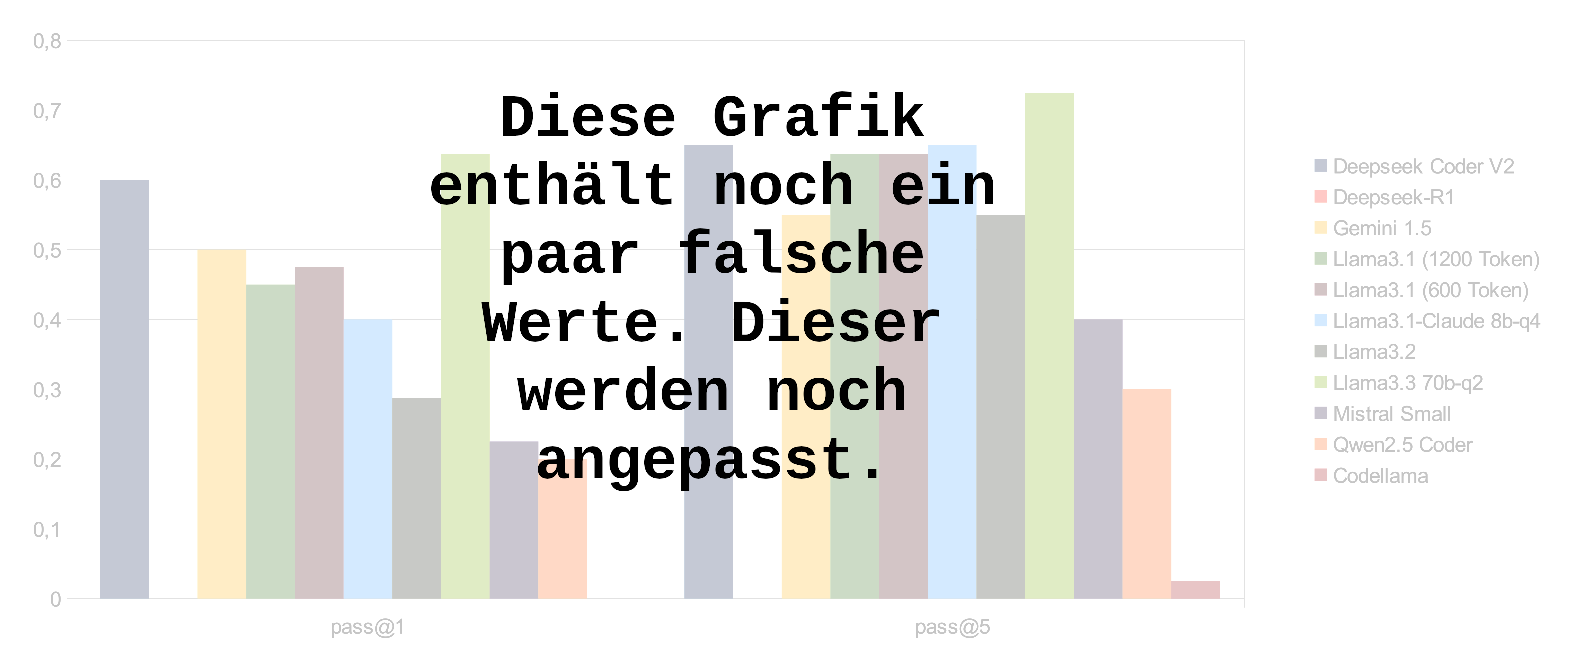
\includegraphics[width=\textwidth]{content/chapter_evaluation/images/llm_evaluation.eps}
	\centering
	\caption{Ergebnisse der pass@k-Methode für die Modelle}
	\label{img:pass_at_k_results_by_llm}
\end{figure}

Ein letztes Modell aus der Llama3 Reihe, das dem Benchmark unterzogen wurde, ist das \textit{Llama3.3 70b-instruct-q2\_K}. Mit einem pass@1 Ergebnis von $0,6275$ und $0,725$ beim pass@5 liefert dieses Modell die besten Ergebnisse. Bei dem vorliegenden Modell handelt es sich um ein Modell mit Quantisierung, was die Größe des Modells auf rund 26 GB reduziert.
Bei diesem Modell wurde einige Komponenten einer 2-Bit Quantisierung unterzogen, bei einer fast gleichbleibenden Ausgabenqualität, weitere Informationen sind \cite{hugging-face-2025} zu entnehmen. Das originale Modell mit ca. 43 GB ließ sich nicht mit den verfügbaren lokalen Ressourcen testen.\vspace{0.2cm}

Das Modell \textit{Deepseek Coder V2 16b} ist ebenfalls aus dem Open-Source-Bereich. Bei der Auswertung des pass@1 liegt das Resultat über den Llama-Modellen 3.1 und 3.2. Deutlich besser ist nur das größere Llama3.3 mit 70b. Bei der Auswertung des pass@5 liegt das Modell mit den Llama 3.1 und 3.2 fast gleich auf. Hier ist nur das Llama 3.3 Modell um 7,5\% besser als DeepSeek-Coder-V2 Modell. Das zweite Modell von der KI-Entwicklungsfirma DeepSeek, welches evaluiert wurde, ist das Modell \textit{DeepSeek-R1}. Dieses Modell hat die besten Ergebnisse erzielt, obwohl es nicht größte von den getesteten Modellen ist. Mit nur 32b liegt es beim pass@1 mit 7,5\% vor dem Llama 3.3 mit 70b und bei der Auswertung des pass@5 sind es 11,5\% vor dem Llama3.3 Modell.\vspace{0.2cm}

Zusätzlich wurden zwei weitere Modelle aus dem Open-Source-Bereich in die Evaluation einbezogen: \textit{Mistral-Small 22b}, entwickelt von der Firma MistralAI, sowie \textit{Qwen 2.5 Coder 32b}. Die Leistung dieser beiden Modelle fiel im Vergleich zu anderen Modellen jedoch geringer aus. Insbesondere lagen die Trefferquoten von \textit{Mistral-Small 22b} und \textit{Qwen 2.5 Coder 32b} bei etwa der Hälfte der durchschnittlichen Trefferquoten der getesteten LLama-Modelle.\vspace{0.2cm}


%Die Antworten von ChatGPT enthielten bei der ersten Abfrage Programmcode, alle weiteren Abfragen verwiesen auf den ersten Prompt. Eine Antwort ist in ?? dar gestellt, diese wurde in ähnlicher Weise immer wieder generiert.
%\hrulefill
%Der Code in deinem Kommentar ist identisch mit dem aktuellen Inhalt. Wenn du Än\-der\-ungen vornehmen möchtest, präzisiere bitte, was angepasst werden soll, und ich werde es umsetzen!
%\begin{flushright}
%	\textit{Generiert von ChatGPT 3.5}
%\end{flushright}
%\hrulefill

Ein weiteres Modell ist Gemini 1.5. von Google und gehört zu den Cloused-Source-Modellen. 

Einige Aufgaben wurden von Gemini aber wie ein Chat behandelt. So hat das Modell Antworten generiert, die einer Konversation mit einem Chatbot ähneln, so wurde beispielsweise der folgende Text generiert, der einen Bezug zur zuvor gegebenen Antwort des Modells herstellt.\vspace{0.2cm}

\hrulefill\vspace{-0.7cm}

\texttt{function greatestCommonDivisorRecursive(\$a, \$b) \{}

\texttt{\hspace{0.6cm} // ... (Rest der Funktion bleibt ähnlich)}

\texttt{\}}\vspace{-0.7cm}

\begin{flushright}
	\textit{Generiert von Gemini 1.5}
\end{flushright}\vspace{-0.7cm}

\hrulefill

Diese generierten Codeausschnitte haben die Tests nicht bestanden und wirken sich somit negativ auf die Auswertung aus.\vspace{0.2cm}


\subsection{Evaluierung nach Sprache}
Eine Überprüfung der Modelle, ob die englische Sprache besser Ergebnisse liefern würde, wurde exemplarisch mit den \textit{Llama}-Modelle \textit{3.1:8b}, \textit{3.2:3b} und \textit{3.3:70b} durch geführt. Alle drei Modelle repräsentieren unterschiedliche Anzahl der Parameter und somit verschiedene Modellgrößen.\vspace{0.2cm}

Da das Training der Modelle in englischer Sprache erfolgt, lag die Vermutung nahe, dass eine Evaluierung in dieser Sprache, wesentlich bessere Ergebnisse liefern sollte. Dies zeigen auch die Auswertungen in \cite[][11]{peng-2024} (Tabelle 12), bei denen die Programmiersprache PHP in der englischen Version im Durchschnitt besser abschnitt.\vspace{0.2cm}

Diese Vermutung konnte mit den durchgeführten Tests der ausgewählten Modelle nur bedingt bestätigt werden. Das Llama3.3 zeigt beim pass@1 einen besseren Wert, in der englische Version. Dieser Wert nähert sich mit steigendem $k$ Wert an, sodass bei $k=5$ die Ergebnisse in Englisch und Deutsch identisch sind. Beim Llama3.2 zeigt das Modell mit einem steigendem $k$-Wert bessere Resultate in der deutschen Sprache. Das Llama3.1 Modell zeigt ein ausgeglichenes Resultat der beiden Sprachen im Vergleich. Hier sind die pass@3 Resultate in Deutsch und Englisch identisch. Während bei abnehmenden $k$-Werten die englischen Resultate besser werden, werden bei zunehmenden $k$-Wert die deutschsprachigen Ergebnisse besser.\vspace{0.2cm}

In der Abbildung \ref{img:pass_at_k_results_by_llama_lang} werden die Ergebnisse der $pass@k$-Methode mit $k=1 … 5$ für die ausgewählten Llama-Modelle zusammengefasst. Die Proben wurden jeweils in Englisch und in Deutsch an die Modelle gestellt.\vspace{0.2cm}

\begin{figure}[!ht]
	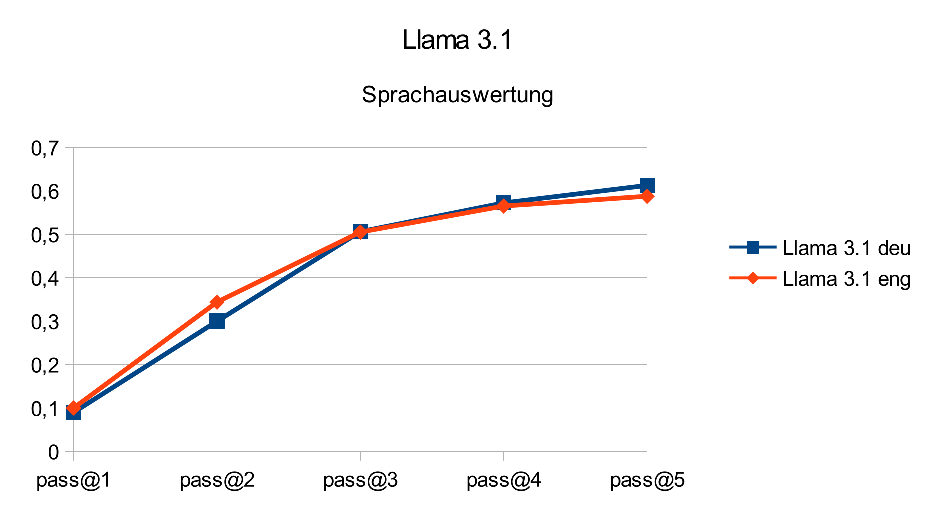
\includegraphics[width=0.45\textwidth]{content/chapter_evaluation/images/llama31_evaluation_lang.eps}
	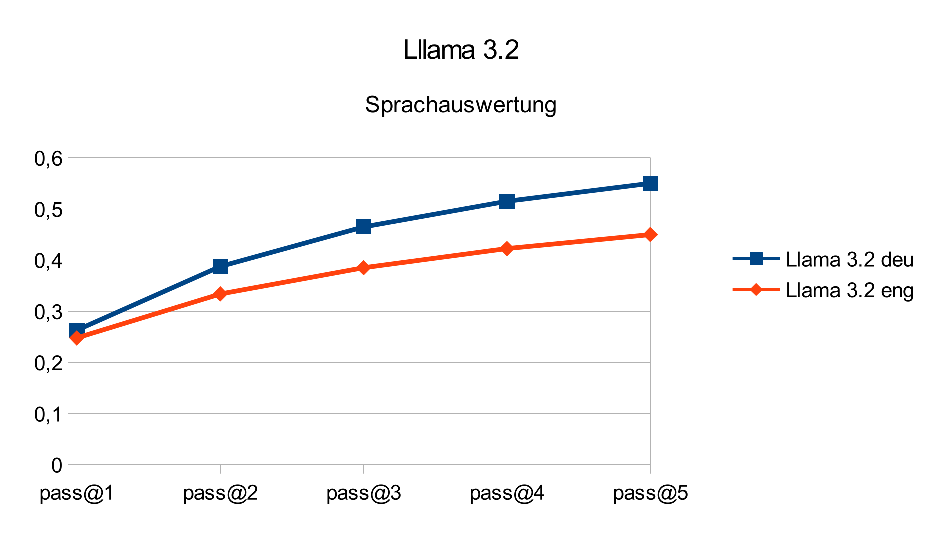
\includegraphics[width=0.45\textwidth]{content/chapter_evaluation/images/llama32_evaluation_lang.eps}
	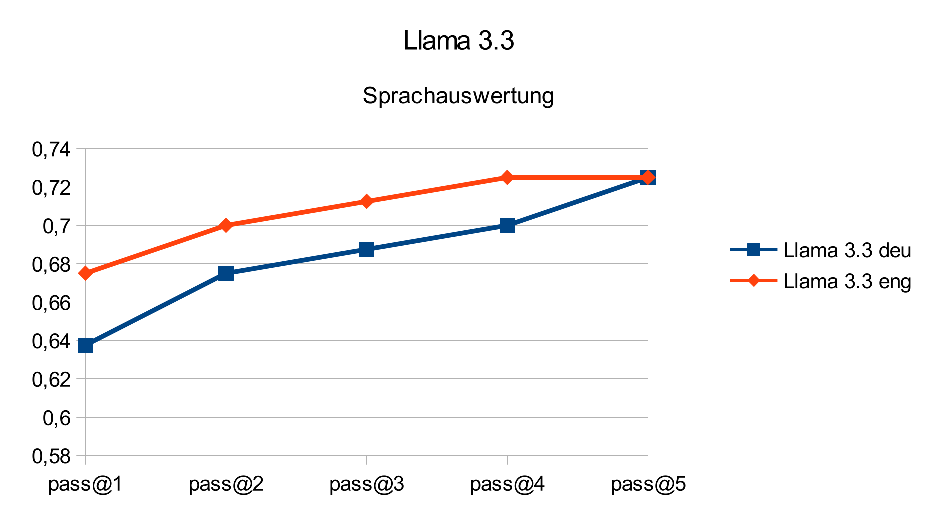
\includegraphics[width=0.45\textwidth]{content/chapter_evaluation/images/llama33_evaluation_lang.eps}
	\caption{Ergebnisse der pass@k-Methode für Llama Modelle verschiedener Sprachen}
	\label{img:pass_at_k_results_by_llama_lang}
\end{figure}

Dieser Test zeigt auch das eine deutschsprachige Verwendung der Modelle nicht zwangsläufig schlechteren Code generieren. Daraus wird der Schluss gezogen, das bei der Optimierung der Prompts eine Übersetzung ins Englische nicht unbedient zu einer signifikanten Verbesserung führt.

\subsection{Nachteile der Evaluierung}\label{subsec:disadvantages_of_evaluation}
Trotz seines Einsatzes bei der Evaluierung von Modellen, zeigt der Benchmark-Test einige Fehler. Dadurch resultieren Nachteile, die sich bei der Bewertung der Modelle negativ auswirken.\vspace{0.2cm}

Einige \textit{\textbf{Fragen sind nicht eindeutig formuliert}} und können von den Modellen falsch interpretiert werden. Ein Beispiel im HumenEval-XL Benchmark ist die Aufgabe 20. Der genaue deutsche Wortlaut ist wie folgt, \textit{Überprüfen Sie, ob zwei Wörter dieselben Zeichen enthalten.}, der gesamte Prompt ist in Listing \ref{lst:humaneval_xl_prompt_20} zu sehen. In der hier durchgeführten Evaluierung wurde diese Aufgabe im \textit{pass@1} nur einmal bestanden. Der Wortlaut hält die Modelle an, einen Vergleich in der Methode selbst durchzuführen. In der, durch den Benchmark vorgegebenen Test, werden aber zwei Zeichenketten verglichen. D.h. als erwartetes Ergebnis sollte eine Zeichenkette erstellt werden, welche die doppelten Zeichen zweier zu testenden Zeichenketten enthält. Das Listing \ref{lst:humaneval_xl_test_20} zeigt einen Teil des Tests und die erwarteten Ergebnisse.\vspace{0.2cm}

\begin{lstlisting}[
	language=php,
	label=lst:humaneval_xl_prompt_20,
	caption={Wortlaut der Aufgabe 20 im HumalEval-XL Benchmark}
]
<?php
/**
* Sie sind ein erfahrener PHP-Programmierer und hier ist Ihre Aufgabe.
* * Überprüfen Sie, ob zwei Wörter dieselben Zeichen enthalten.
* >>> same_chars('eabcdzzzz', 'dddzzzzzzzddeddabc')
* True
* >>> same_chars('abcd', 'dddddddabc')
* True
* >>> same_chars('dddddddabc', 'abcd')
* True
* >>> same_chars('eabcd', 'dddddddabc')
* False
* >>> same_chars('abcd', 'dddddddabce')
* False
* >>> same_chars('eabcdzzzz', 'dddzzzzzzzddddabc')
* False
*/
function sameChars($s0, $s1){
\end{lstlisting}

\begin{lstlisting}[
	language=php,
	label=lst:humaneval_xl_test_20,
	caption={Wortlaut des Tests 20 im HumalEval-XL Benchmark}
]
function compare($x, $y) {
	return $x == $y;
}

$arg00 = "eabcdzzzz";
$arg01 = "dddzzzzzzzddeddabc";
$x0 = sameChars($arg00, $arg01);
$v0 = true;
if (!compare($x0, $v0)) {
  throw new Exception("Error at 1th assert statement.");
}
\end{lstlisting}

Eine weitere Fehlerquelle ist das \textit{\textbf{Zusammenführen der Antworten der Modelle und Tests aus dem Benchmark}}. Meist ist das Problem das Parsen der Sonderzeichen, wie beispielsweise die Verwendung der doppelten Anführungszeichen im Test und den erstellten Antworten. Eine manuelle Prüfung der Aufgabe 2 hat das Fehlverhalten aufgezeigt. Durch den Einsatz einer weiteren Pythoncodezeile, wie in Listing \ref{lst:error_evaluation_code_1} zeigt konnten die Bewertung einiger Modelle verbessert werden. So hat sich die Bewertung für das \textit{pass@1} des Deepseek-Coder-V2 um 7\% von $0,53$ auf $0,6$ verbessert. Ebenso wurde für das Llama3.1 Modell eine Verbesserung von $0,45$ auf $0,475$ ermittelt.\vspace{0.2cm}

\begin{lstlisting}[
	language=diff,
	label=lst:error_evaluation_code_1,
	caption={Fehler bei der Auswertung durch fehlerhafte Anführungszeichen}
]
  answer = answer.replace(r"\n", "\n")
+ answer = answer.replace(r'\"', '"')
+ 
+ test = test.replace(r'\"', '"') 
\end{lstlisting}

Bei der Probe \textit{php/5} wurde eine \textit{\textbf{fehlerhafte Übersetzung}} festgestellt. So wurde die Probe übersetzt, nicht aber die Tests. Das Listing \ref{lst:prompt_php_de_5} zeigt die gültigen Werte welche als Eingabeparameter für die zu generierende Funktion erlaubt sind. Hier handelt es sich um deutsche Zahlworte von $null$ bis $neun$.\vspace{0.2cm}

\begin{lstlisting}[
	language=php,
	label=lst:prompt_php_de_5,
	caption={Aufgabenstelleung der Probe php/5}
]
/**
* Sie sind ein erfahrener PHP-Programmierer und hier ist Ihre Aufgabe.
* Die Eingabe ist ein durch Leerzeichen getrennter String von Ziffern von 'null' bis 'neun'.
*     Gültige Optionen sind 'null', 'eins', 'zwei', 'drei', 'vier', 'fünf', 'sechs', 'sieben', 'acht' und 'neun'.
*     Gib den String mit den Zahlen sortiert von klein nach groß zurück.
* >>> sort_numbers('three one five')
* 'one three five'
*
*/
function sortNumbers($numbers){
\end{lstlisting}

Der Test der Probe \textit{php/5}, welcher in Listing \ref{lst:test_php_de_5} zu sehen ist, erstellt eine Prüfung der generierten Methode mit englischem Zahlworten von $zero$ bis $nine$ bereit. Keines der getesteten Modelle hat diese Probe bestanden.

\begin{lstlisting}[
	language=php,
	label=lst:test_php_de_5,
	caption={Aufgabenstelleung der Probe php/5}
	]
// more tests.

$arg40 = "six five four three two one zero";
$x4 = sortNumbers($arg40);
$v4 = "zero one two three four five six";
if (!compare($x4, $v4)) {
	throw new Exception("Error at 5th assert statement.");
}
\end{lstlisting}

Die Tests aus dem Benchmark und Ergebnisse der Modelle wurde stichprobenartig manuell geprüft und weitere Fehler behoben. Dennoch ist nicht auszuschließen das die jetzige Evaluation weitere Fehlerquellen enthält.\vspace{0.2cm}

Es gibt durchaus weitere Fehlerquellen, welche die Ergebnisse negativ beeinflussen können. Bei der Formulierung der Tests könnten Randbedingungen nicht korrekt betrachtet wurden sein, was dazu führen kann, dass der Einsagt der generierten Codes zu Fehlern führen könnte. Ebenfalls können die Tests falsche Parameter vorgeben, wodurch korrekt generierter Code als falsch bewertet wird. Die eben genannten Fehler konnten im vorliegenden Ergebnissen nicht nachgewiesen werden, ganz auszuschließen sind sie aber nicht.

%--- Optimierung -----------------------------------------------------------------------------------


\section{Optimierung der Eingabeaufforderungen}
% https://ki-techlab.de/ki-news/evaluierung-grosser-sprachmodelle-ein-technischer-leitfaden/
Als Ziel der Optimierung gilt das die LLMs effizienten, präzisen und korrekten Code zu generieren. Ein Ansatz dies zu erreichen ist die Prompts zur Codegenerierung mithilfe einer LLMs zu erstellen oder zu verbessern.

\begin{tcolorbox}[
	enhanced,
	colback=red!5!white,
	colframe=red!75!black!50,
	title= Mein roter Faden
	]
	Hier kommen noch Optimierungsangaben, die stehen zurzeit nicht fest.
\end{tcolorbox}


\subsection{Optimierung durch Framework}
Ergebnisse der Optimierung durch die Auswahl des Frameworks.

\begin{figure}[!ht]
	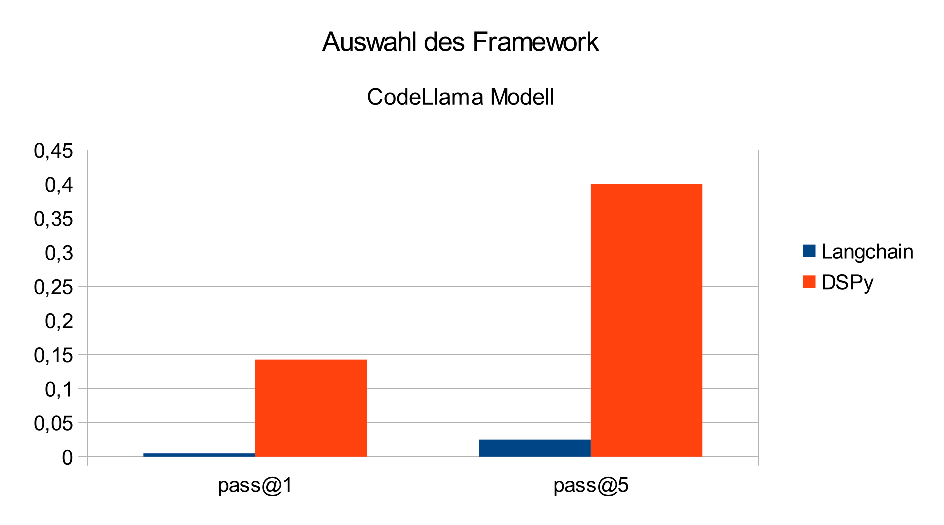
\includegraphics[width=0.5\textwidth]{content/chapter_evaluation/images/framework_evaluation_codellama.eps}
	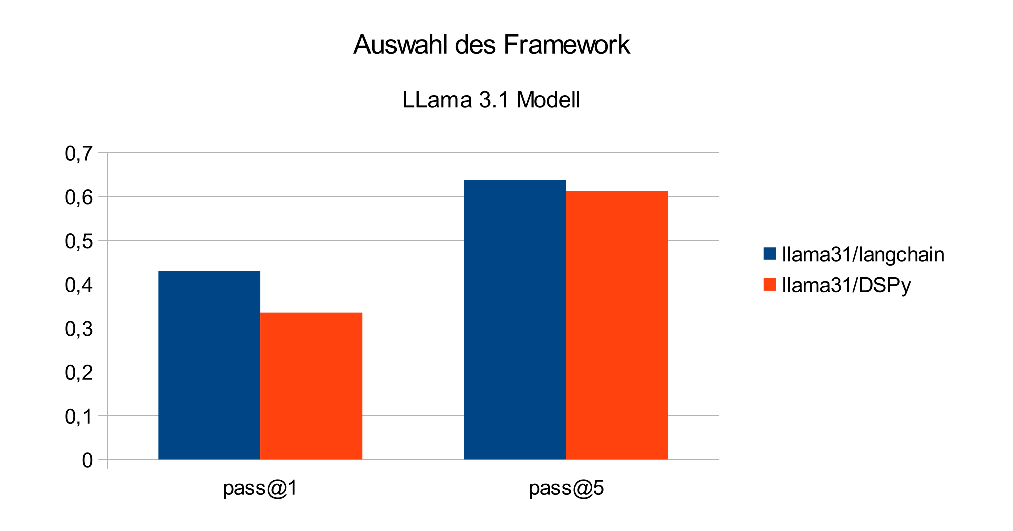
\includegraphics[width=0.5\textwidth]{content/chapter_evaluation/images/framework_evaluation_llama31.eps}
	\caption{Ergebnisse der pass@k-Methode für unterschiedliche Frameworks}
	\label{img:pass_at_k_results_by_framework}
\end{figure}

